\documentclass[Report.tex]{subfiles}

\begin{document}

\begin{figure}
\center
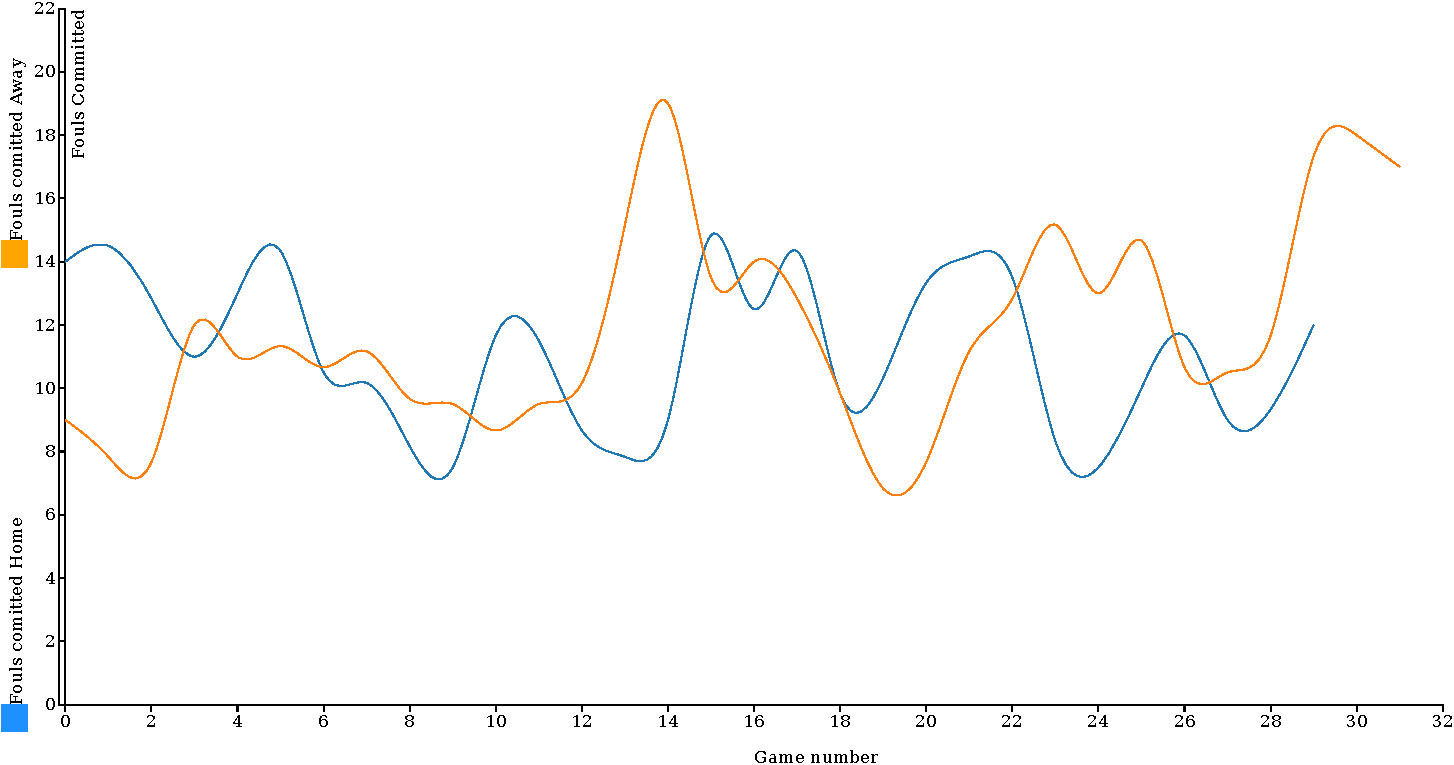
\includegraphics[scale=0.6]{Figures/fouls.pdf}
\caption{}
\label{Fig:}
\end{figure}


\subsubsection{What-why-how}
In hopes of discovering a trend between how far in a season a team is, and how many fouls they commit, we plotted these two variables together. A choice was made to separate matches where the teams are home, and the matches where they are not. This was done because there could be a difference in confidence and play-style, as well as there not being the same amount of matches played home and away.
 As seen on the chart, there is a lot of rising and falling. In order to conclude anything, alot more data would be needed than the few seasons we have access to at this point. However, the rising and falling could indicate difference in aggressiveness based on what team is their opponent in the match, we haven't quite gone deep enough go give any definitive answers as to what teams they in general prefer to be aggressive against.

\subsubsection{Code}
The code behind this chart lies in gathering and processing statistics for a team over multiple rounds, then filtering it for everything else than the foul statistics, while still preserving the right order of the matches. After that is done, it is put in D3, with some relatively simple code for a line chart.


\end{document}
